\chapter{Introduction} \label{chapter1}

Population geneticist are historians telling the story of evolution. Mutation and recombination leave faithful historical records in the genome of every single organism on earth. The records have always been there, but over the past decades, the experimental and computational tools to decipher those records have improved dramatically. This introductory chapter surveys several key methodological trends that have transformed population genetic research, and finally delineates how these trends have built up the momentum for the original work presented in this thesis.

\section{Genealogical modeling of evolution using the \acl{ARG}} \label{intro-arg}

%% Intro from pedigree to ARG, explain coalescence and recombination
The genetic relationships between ancestors and descendants form the basis of all evolutionary genomics research. The simplest data structure that encodes ancestor-descendant relationships is a pedigree (light grey in Fig. \ref{fig:intro-F1}A), commonly known as a ``family tree". The pedigree is a graphical structure representing genealogical ancestry of individual organisms. During meiosis in sexually-reproducing diploid organisms, any given position in a haploid gamete is randomly sampled from either chromosome through meiotic recombination. Consequently, the pedigree alone cannot fully specify the genetic ancestry of every position in the genome. Since random shuffling of parental chromosomes through recombination creates a mosaic of genetic ancestry along the genome, different non-recombining segments of the genome have different paths of genetic inheritance in the pedigree. The collection of all paths (or lineages) along which inherited segments of the genome have been transmitted forms a complex graphical structure embedded in the pedigree known as an \acf{ARG} (dark grey in Fig. \ref{fig:intro-F1}A, \cite{griffiths1997progress}). The \ac{ARG} is a \textit{complete} record of the history of genetic inheritance for a set of sampled genomes (solid nodes \textcircled{A}, \textcircled{B}, \textcircled{C} and \textcircled{D} at the tips of the \ac{ARG} in Fig. \ref{fig:intro-F1}).

\begin{figure}%[h]
    \centering
    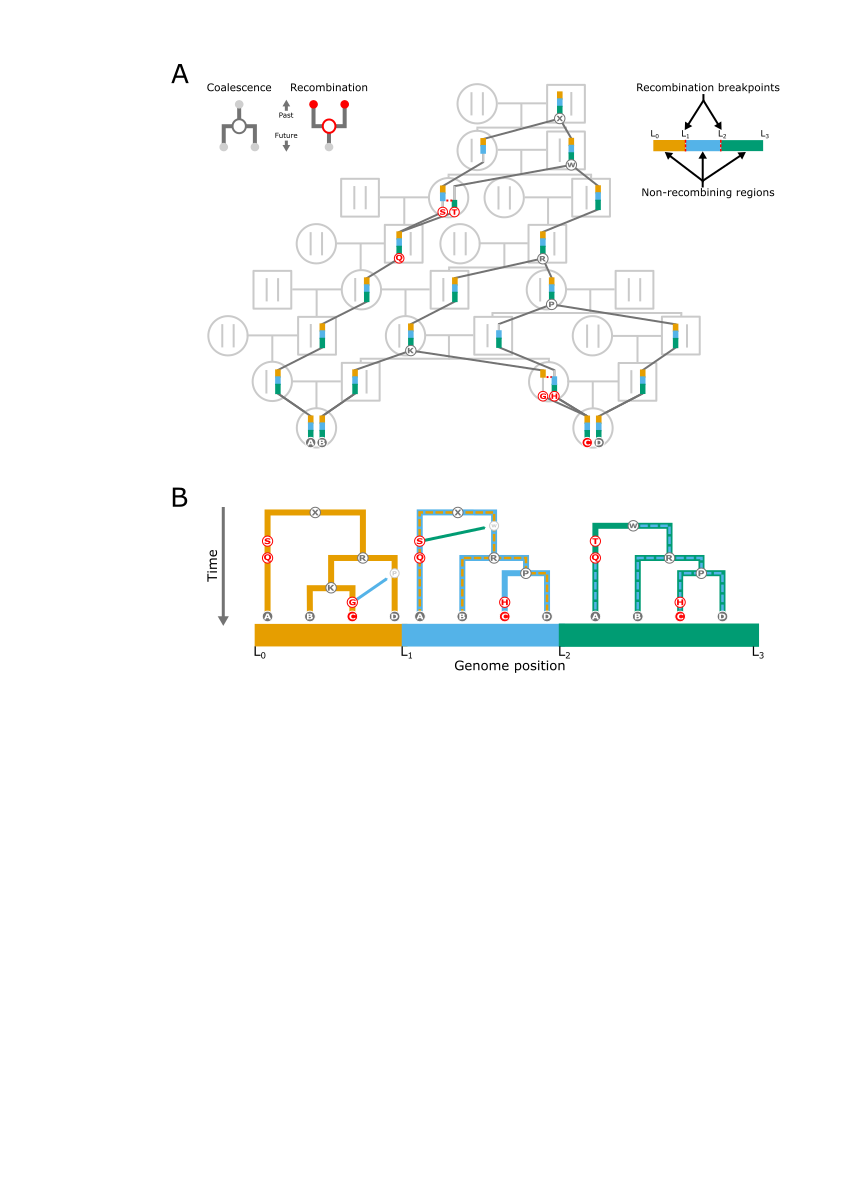
\includegraphics[width=\textwidth]{adapted_figs/arg_illustration.png}
    \caption[A simple example of an \acf{ARG}]{\textbf{A simple example of an \acf{ARG}}. (\textbf{A}) An \ac{ARG} (dark grey) embedded in a pedigree (light grey). Each node of the pedigree corresponds to an individual organism, connected by edges representing parent-offspring relationships. Each node of the \ac{ARG} corresponds to a haploid genome, connected by edges representing genetic inheritance between an ancestor and a descendant. Note that the example here assumes the samples are from the nuclear genome of sexually-reproducing diploid organisms, which is the most common scenario of interest. (\textbf{B}) An alternative representation of the \ac{ARG} in (\textbf{A}) as a series of local genealogies that share nodes and edges. The arrows represent \acf{SPR} operations associated with recombination events that convert local genealogies to their rightward neighbor. The dashed lines highlight each tree's shared structure with its leftward neighbor. Figure adapted from \cite{lewanski2023era} under a \href{https://creativecommons.org/licenses/by/4.0/}{CC BY 4.0} license.}
    \label{fig:intro-F1}
\end{figure}

Bifurcating nodes in an \ac{ARG} represent two types of events -- coalescence and recombination. A node where two edges enter from the future but only a single edge exit to the past represents when two lineages find common ancestry and \textit{coalesce} into a single lineage backward in time (e.g. grey coalescence nodes \textcircled{K}, \textcircled{P}, \textcircled{R}, \textcircled{W} and \textcircled{X} in Fig. \ref{fig:intro-F1}). Forward in time, a coalescence event occurs through a parent providing the same copy of genomic segment to multiple descendants. Conversely, a node where a single edge enter from the future but two edges exit to the past represents a single lineage of a \textit{recombinant} offspring from two parental lineages (e.g. red recombination nodes \textcircled{C} and \textcircled{Q} in Fig. \ref{fig:intro-F1}). Forward in time, a recombination node corresponds to a parent passing on a haploid gamete resulting from recombination between its two haploid genomes.

% talk about tree representation
The \ac{ARG} additionally records the age of each node (not labeled in Fig. \ref{fig:intro-F1}) as well as the position of the recombination breakpoint (dashed red lines in Fig. \ref{fig:intro-F1}) associated with each recombination node. Therefore, the full genealogy of every non-recombining genomic region can be constructed by traversing the the \ac{ARG} backwards in time and following the lineage on the appropriate side of the recombination breakpoint. The correspondence between the full \ac{ARG} and local genealogies naturally leads to an equivalent representation of an \ac{ARG} as a series of genealogical trees along the genome with shared nodes and edges (Fig. \ref{fig:intro-F1}B). Each local tree encodes the evolutionary history of a non-recombining genomic segment and can be transformed into the next one by removing a single edge and attaching it to a different node (arrows in Fig. \ref{fig:intro-F1}B). This operation termed \acf{SPR} reflects the outcome of a recombination event manifested in local genealogies. The graphical representation of a full \ac{ARG} can be recovered by sequentially combining the shared nodes and edges of each local tree while annotating each recombination node with its breakpoint position. In practice, the tree-sequence form of the \ac{ARG} (see \ref{intro-sim}) is frequently used both as the output of inference algorithms and input for downstream applications (\cite{lewanski2023era}), due to not only its tractability, but also the spatially local nature of many population genetic inference problems (such as identifying sites or region under selection).

%% Utilities of ARGs, give some examples of how problems can be formulated as questions about the ARG, mention sum stats
The \ac{ARG} constitutes the complete record of ancestral information among a set of genomes. Evolutionary processes such as selection, drift and gene flow all have a direct impact on the structure of an \ac{ARG}. Consequently, many population and evolutionary genetic questions can be formulated as inquiries into the \ac{ARG} (\cite{rasmussen_genome-wide_2014,lewanski2023era}). For example, the rate of coalescence reflected by the \ac{ARG} is informative of the effective population size over time, whereas the distribution of recombination breakpoints in the \ac{ARG} is directly tied to recombination rate across the genome. Furthermore, under the infinite sites model, samples of genomic sequences are stochastic readout of the \ac{ARG} through a Poisson process of mutations (\cite{wakeley2005coalescent}). Thus, any quantity or statistic derived from the genomic sequences (e.g. the \acs{SFS}, $F_{\mathrm{ST}}$, $\pi$, $\theta$, heterozygosity etc.) is but a low-dimensional summary of the underlying \ac{ARG} (\cite{ralph2020efficiently}). While these summary statistics have demonstrated great utility in providing meaningful evolutionary insights, the \ac{ARG} holds much richer information that can be tapped into for evolutionary analyses.

%% ARG inference methods

Although the \ac{ARG} is a powerful theoretical and conceptual tool to crack the code of evolution, in practice it must be inferred from population genomic data. \ac{ARG} inference has historically been a very challenging problem (\cite{rasmussen_genome-wide_2014,mathieson_what_2020}). The search space of all possible structures of an \ac{ARG} grows rapidly with increasing genome and sample sizes. In addition, as mentioned previously, the observed genomic sequences are noisy readout of the true \ac{ARG}. Mutation creates concordant patterns of genetic variation from which \acp{ARG} can be inferred, whereas recombination breaks up such patterns and reduces the amount of information per genealogy. The opposing forces of mutation and recombination impose a limit on \ac{ARG} identifiability from genomic sequences (\cite{hubisz2020inference,hayman2023recoverability}), which in turn limits the utility of \acp{ARG} in downstream applications. Early methods aimed to built a parsimonious \ac{ARG} that contains the minimal number of recombination events given a genotypic matrix (\cite{wong2023general}), which is a NP-hard problem (\cite{wang2001perfect}). These methods therefore rely on heuristics and are limited in scale of their applications. Recently, there has been great stride towards accurate \ac{ARG} inference at a practical scale. ARGweaver (\cite{rasmussen_genome-wide_2014}) and its extension ARGweaver-D (\cite{hubisz_mapping_2020}) mark the inception of statistically rigorous genome-wide \ac{ARG} inference. ARGweaver introduces a novel technique termed “threading” which adds an $n$-th sequence to an existing \ac{ARG} of $n-1$ sequences under a likelihood model defined by \iac{HMM}. The state space of the \ac{HMM} is simplified using approximations of the coalescent and discrete time to make the ``threading" operation a computationally tractable sampling step from the posterior distribution of \acp{ARG} using \ac{MCMC}. ARGweaver can be applied to up to a hundred whole genomes and remains the state of the art in terms of accuracy (\cite{brandt2022evaluation}). With the rapid growth of modern biobank-scale genomic datasets, a number of methods that balances statistical rigor and computational efficiency have been developed, such as Relate (\cite{speidel_method_2019}) and tsinfer/tsdate (\cite{kelleher_inferring_2019,wohns_unified_nodate}). These methods employ various heuristics and simplifications and consequently tend to underestimate recombination and only provide point estimates of the \ac{ARG} (\cite{lewanski2023era,wong2023general}), but have the remarkable ability to scale up to tens or even hundreds of thousands of genomic samples (see \cite{brandt2022evaluation} for a benchmark and comparison of prevailing inference methods). The suite of \ac{ARG} inference tools with a spectrum of accuracy-scalability tradeoffs has paved the way for a new generation of methods that tackle a variety of empirical questions in population genetics (\cite{stern_approximate_2019,stern_disentangling_2021,speidel_method_2019}).

\section{Population-genetic simulations power large-scale \textit{in silico} experiments of evolution} \label{intro-sim}

%% Types of simulations: fwd vs. coal -> hybrid/ recapitation, accelerate
Without the ability to rewind time, we cannot observe evolution occur in real time in natural populations (barring some rare exceptions of feasible large-scale experimental evolutionary studies in species with short generation times). In most cases, \textit{in silico} simulations provide the only way to replay various evolutionary scenarios and conduct experiments of evolution. Population simulators are therefore an indispensable tool across all aspects of population genetic research ranging from validating theoretical expectations, testing hypothesis to powering Monte Carlo methods.

The process of simulating the evolution of a population may seem straightforward. We can simulate the reproduction of every individual in the population according to some model of choice, most commonly the Wright-Fisher model (\cite{wakeley2005coalescent,hahn2018molecular}). The simulation runs forward in time for many generations while mutation and recombination processes are recorded in the genomes of extant individuals at each generation. In the end, to generate one simulated dataset, some number of individuals and their genomes are sampled from the latest generation. This \textit{forward} simulation approach can be very flexible since it is facile to incorporate a wide range of evolutionary processes such as different forms of natural selection, complex demographic history or migration patterns into the simulations (\cite{hahn2018molecular}). However, forward simulations can become unwieldy in practice. First, since each individual needs to be tracked every generation, the amount of computation scales with the population size $N_e$, which is not uncommon to be quite large. In addition, simulations need to run until the population reaches equilibrium, which usually takes a number of generations on the order of the long-term $N_e$ (\cite{wakeley2005coalescent}). Hence, forward simulations scale approximately quadratically with the population size.

Researchers have come up with two types of techniques to circumvent the computational challenge. At its heart, population genomic simulations are simulations of the \ac{ARG} (see \ref{intro-arg}). Given a particular mutation model, neutral genetic variations in the genome are strictly governed by the \ac{ARG} (\cite{wakeley2005coalescent,hahn2018molecular}). Therefore, it is not necessary to generate neutral mutations during forward simulation. They can be overlaid onto the genealogies under a mutation model of choice to generate genomic sequences post hoc. The forward simulator SLiM (\cite{haller_slim_2019}) employs this tree-sequence recording procedure (\cite{haller_tree-sequence_2019}, also see below) to improve computational efficiency. Another key observation of the forward simulation process is that many historical individuals do not turn out to be genetic ancestors to the contemporary population from which the samples are taken. Therefore, if we take a \textit{backwards}-in-time approach, start from a sample of contemporary individuals and generate only the ancestors of these samples, we can avoid the computational burden of keeping track of the entire population every generation. This can be accomplished by sampling ancestral lineages under the coalescent process (\cite{kingman1982coalescent,kingman1982genealogy,hudson_gene_1990,tajima1983evolutionary}). The coalescent is an approximation of a forward Wright-Fisher population under the key assumption $N_e >> n$, where $N_e$ is the effective population size and $n$ the sample size. This assumption holds for many realistic use cases and therefore coalescent simulators provide a highly efficient way to generate population samples at scale. Coalescent simulations trade flexibility for computational efficiency. Early coalescent simulators were limited to only neutrally evolving populations (\cite{hahn2018molecular,lewanski2023era}). However, a new generation of coalescent simulators have emerged with the ability to handle more complex demographic scenarios and some form of selection. Among these, discoal (\cite{kern_discoal_2016}) and msprime (\cite{kelleher2016efficient}) have been most widely adopted to simulate biologically realistic samples at a practical scale.

A key innovation that has further revolutionized evolutionary simulations is the introduction of a \textit{hybrid} approach that exploits the strengths of both forward and backward (coalescent) simulators. The overall idea is to perform the more complex portion of the simulation where biological realism is paramount (e.g. population under various modes of selection) with a forward simulator and leave the simpler or less important portion (e.g. neutrally evolving population) to a coalescent simulator. This can be accomplished through either ``recapitation" of uncoalesced lineages in the first generation of a forward simulation until \iac{MRCA} is found with a coalescent simulator (\cite{haller_slim_2019}), or using a complete coalescent simulation to initialize a population and carry on the simulation with a forward simulator. This approach has been popularized thanks to the tskit python API (\cite{kelleher2016efficient,kelleher2018efficient}), which provides an interoperable data structure (ts format) for the tree-sequence encoding of the \ac{ARG}. The ts format is flexible, has a low storage footprint, and therefore has fostered an ecosystem of software tools along the simulation, inference and analysis pipeline of population genetic research.

Finally, it is worth mentioning that a community-driven effort to maintain a catalog of simulation models and a high-level API to simulate under these models out-of-the-box has emerged (\cite{adrion_community-maintained_2020,lauterbur_expanding_2022}). The stdpopsim project has made efficient large-scale simulations of complex evolutionary scenarios ever more accessible. The advancement of the simulation infrastructure has ultimately opened up opening up new opportunities and avenues for population genetic research, such as using simulations to generate perfectly labeled training data for supervised machine learning models.

\section{Deep learning methods for population genetics} \label{intro-DL}

%% historical perspective, model-based, data lag behind => Methods lag behind, more data driven
Population genetics is a century-old discipline that arose long before the era of genomics. Over the 20\textsuperscript{th} century, a rich body of theory has emerged that aims to describe how the interplay among different evolutionary forces (such as mutation, recombination, selection, drift and gene flow) shapes the population dynamics of genetic variants. This tradition of probabilistic and statistical modeling led to the creation of many mathematical approaches to infer evolutionary parameters from observed patterns of genetic variation even before molecular genetic data became readily available (\cite{korfmann_deep_2023}). Traditional computational methods for population genetic inference (see \cite{marjoram2006modern} for a detailed review) typically employ likelihood-based statistical approaches, such as maximum likelihood, Bayesian or Monte Carlo method to fit an evolutionary model, commonly derived from the Wright-Fisher model or the coalescent (see \ref{intro-sim}), to empirical data for parameter estimation. Traditional statistical approaches have dominated the field because of their interpretability. Since they are rooted in mechanistic or at least generative models of evolutionary processes, traditional methods can often be teased apart under population genetics theory to further our understanding of the molecular genetic mechanism of evolution.

The explosion of massive genomic datasets (e.g. 1000 Genomes Project [\cite{auton_global_2015}], Allen Ancient DNA Resource [\cite{mallick2023allen}], UK Biobank [\cite{sudlow_uk_2015}], 1001 Genomes Project [\cite{alonso20161}]) with the advent of high-throughput sequencing technologies has shifted the bottleneck of population genetic inference from the lack of data to the need for highly scalable and robust computational methods. Traditional model-based statistical methods rest on the assumption that the model sufficiently describes the data (\cite{schrider_supervised_2018}). However, such probabilistic models more or less simplify complex evolutionary processes and sacrifice biological realism for computational tractability in practical applications. These simplifications may be appropriate when each evolutionary force is studied in isolation, but severely limit the utility of traditional statistical methods in deciphering complex evolutionary scenarios from the plethora of genomic data. In addition, the growing size and dimension of population genetic datasets pose a direct challenge to the computational efficiency of traditional methods. Popular algorithms for fitting probabilistic models to molecular genetic data such as \acf{MCMC} and \ac{EM} scale poorly with sample size (\cite{korfmann_deep_2023}). \Acf{ABC}, a widely used method in population genetics for bypassing the calculation of intractable likelihood functions, suffers from ``the curse of dimensionality" in that the approximation error increases with the growing number of summary statistics necessitated by high-dimensional data (\cite{prangle2018summary}). Therefore, while traditional inference methods established from population genetics theory have been successful in yielding valuable evolutionary insights from small-scale molecular markers, the emergence of modern biobank-scale genomic datasets has inevitably transformed population genetics from a theory-driven discipline to a data-driven one.

%% Machine learning and deep learning
\Acf{ML} has demonstrated state-of-the-art performance over a wide range of empirical applications involving big data and become increasingly dominant in all areas of quantitative research. \ac{ML} methods are particularly successful in tackling problems for which large amount of data exist but no analytical solution is available or practical, such as \ac{CV} and \ac{NLP} (\cite{huang_harnessing_2023}). \ac{ML} algorithms are designed to automatically extract informative patterns in the data without explicit parametric models of the data and find solutions to specific inferential tasks. There has been several well-established applications of \ac{ML} to population genetics. For example, \acfp{HMM} are widely used to segment genomic sequences and estimate ancestry (\cite{li2003modeling}) or other evolutionary parameters (\cite{kern2010population,siepel2005evolutionarily,boitard2009detecting,felsenstein1996hidden}) along chromosomes, whereas \acf{PCA} has become an essential tool to visualized high-dimensional genotypic matrices in low-dimensional clusters to inform relatedness among individuals (\cite{schrider_supervised_2018}). These are examples of \textit{unsupervised} \ac{ML} where the model finds structure within the data without prior knowledge of labels provided by humans. \textit{Supervised} \ac{ML}, on the other hand, relies on training data with known labels to make predictions about new datapoints and does so by optimizing model parameters to maximize the prediction accuracy of a response variable from the input. The application of supervised \ac{ML} is relatively new to the field of population genetics and was introduced by \cite{pavlidis2010searching}, where they addressed the lack of evolutionary ground truth (\ref{intro-sim}) by utilizing synthetic training data generated via simulations. 

The advancement in deep learning has an outsized impact on the success of the supervised \ac{ML} paradigm. Deep learning uses neural networks with nodes in multiple layers that are capable of many possible mathematical operations and can therefore learn a deep hierarchical representation of the data. During training, the connection weights between nodes are optimized to minimize the loss usually defined by the prediction error. Neural networks are universal function approximators that automatically learn complex features from raw data and thus provide exceptional performance on prediction tasks across a wide range of domains (\cite{lecun_deep_2015}). The rest of this section will briefly examine the major neural network architectures with a focus on supervised deep learning models for predictive tasks (other learning paradigms in population genetics are reviewed by \cite{huang_harnessing_2023,korfmann_deep_2023}, see also \ref{evo-genAI} for discussion of the most recent developments in generative models).

% different ML archs with context of popgen apps: FNN, CNN, RNN, newer transformer, cf. concl.
\Acp{FNN} are the archetypal architecture of deep learning models. A vector of input features enters the \ac{FNN} via the input layer, which is connected to the output layer via a series of hidden layers. Each layer receives output from the previous layer and applies some form of non-linear transformation through activation functions before passing its output to the next layer. Under the Universal Approximation Theorem, \acp{FNN} can approximate any continuous function to any desired precision and therefore are suitable for many generic prediction tasks (\cite{korfmann_deep_2023}). A notable early adoption of \acp{FNN} in population genetics is the evoNet model that jointly infers selection and demography from summary statistics (\cite{sheehan_deep_2016}). \acp{FNN} have subsequently been applied to various problems such as inferring mutation rates, population structure or admixture events (\cite{huang_harnessing_2023}).

\Acfp{CNN} are uniquely suited for genomic applications as they are specifically designed to handle grid-like input. Originally proposed to process image data, \acp{CNN} are widely adopted for \ac{CV} tasks such as image classification or segmentation (\cite{lecun_deep_2015}). \acp{CNN} consist of consecutive sets of convolutional and pooling layers. Each convolutional layer uses a set of kernels (or filters) to generate feature maps of its input through convolution operations, and the subsequent pooling layer reduces the size of the feature maps by combining information from adjacent regions. It is straightforward to treat genotype or haplotype sequences as images and \acp{CNN} have indeed been utilized in this manner for inferring demography (\cite{flagel_unreasonable_2019,sanchez2021deep}), local ancestry (\cite{montserrat2020lai,sabat2022salai}), selection (\cite{flagel_unreasonable_2019,torada_imagene_2019}), introgression (\cite{blischak2021chromosome,gower2021detecting,ray2023introunet,zhang2023inferring}) and recombination (\cite{adrion_predicting_2020}).

Another deep learning architecture tailored to specific input format are \acfp{RNN}. \acp{RNN} incorporate a mechanism that allows the output of a layer to flow back to a previous or current layer and thereby are capable of retaining information from previous inputs. At each stage the current input and the previous output can be combined to produce the next output. The iterative nature of an \ac{RNN} makes it suitable for handling sequential inputs such as speech or text, although novel architectures based on the transformer (\cite{attention2017_3f5ee243}) have emerged as the state of the art for \ac{NLP} tasks (see \ref{evo-genAI}). In the context of population genetics, the input data could be spatially sequential along biological sequences or temporally sequential along evolutionary time. \acp{RNN} have been used for genome-wide estimation of coalescence rate (\cite{khomutov2021deep}) and recombination landscape (\cite{adrion_predicting_2020}).

There are rich opportunities for deep learning approaches to drive profound scientific discoveries in the genomic era, especially in light of the recent success of generative \ac{AI} models (discussed in \ref{evo-genAI}). Within the supervised learning paradigm, two challenges for building accurate and robust deep learning models in population genetics stand out. First, deep learning models so far take either summary statistics or raw genotypic data as input. Given that \acp{ARG} are the ultimate record of evolution but difficult to model analytically (see \ref{intro-arg}), can we take advantage of deep learning models to perform inference from the \ac{ARG}? Second, since most deep learning models in population genetics rely on synthetic data for training, inference on real data is prone to be biased by ill-defined simulation model. This ``simulation mis-specification problem" remains a major concern about current applications of deep learning in population genetics (\cite{korfmann_deep_2023}) and calls for a timely solution.

\section{Studies of selective sweeps generate key insights into adaptive evolution}

The ability to accurately detect and quantify the influence of natural selection from genomic sequencing data is one of the main pursuits in population genetics. Studies of natural selection aim to tackle questions ranging from the genetic basis of historical evolutionary events to the functional and disease relevance of genetic variants in both human and non-human contexts (\cite{karlsson2014natural,henry2014exploring}). Selection can be broadly categorized into different modes, including positive selection, where an allele is favored and increases in frequency, negative selection (or purifying selection), where deleterious alleles are removed from the genome, and balancing selection, where multiple alleles are actively maintained at an appreciable frequency (\cite{vitti2013detecting}).

Adaptive evolution, at the molecular level, is driven by selection acting on alleles that enhance organismal fitness, thereby increasing their frequency in a population (\cite{vitti2013detecting}). Alleles under positive selection often carry important phenotypic relevance and therefore are of particular interest. For example, genome-wide scans of positive selection in human have identified immune-related alleles (e.g. in genes encoding signal transducer of inflammatory response) implicated in pathogen resistance (\cite{fumagalli2011signatures}). These immune-related variants may have therapeutic relevance for both infectious diseases and autoimmune diseases. Studies of selection in plants have also identified alleles associated with adaptation to biotic and abiotic stress, potentially leading to breeding strategies that help create crops resilient to adverse conditions caused by climate change (\cite{henry2014exploring}). 

Population genetics methods identify positive selection through the detection of selective sweeps, which are genomic signatures of positive selection at the population level. A hard sweep is the classic case where a \textit{de novo} beneficial allele rapidly increases in frequency due to selection. A soft sweep differs from a hard sweep in that selection acts on a standing genetic variant rather than a \textit{de novo} mutation. More recent works have started to elucidate cases of polygenic selection in the human genome (\cite{berg2014population,racimo2018detecting,edge2019reconstructing}), which is a more complex scenario of positive selection where selection of a trait acts simultaneously on many variants across the genome. Traditionally, methods to detect selective sweeps take advantage of the hitchhiking effect, where the neutral alleles around the site under selection that are linked to the beneficial allele “hitch-hike” to high frequency. The hitchhiking effect leads to a characteristic reduction of genetic diversity in the vicinity of the site under selection, manifested in both the \ac{SFS} and the haplotype structure. The hitchhiking effect can be captured by specifically designed summary statistics to make inferences about selection. Newer approaches to detect selection include likelihood-based statistical methods and more recently machine learning methods are increasingly adopted for selection inference. Despite many advances, major limitations remain in the sensitivity and scalability of computational methods for identifying and characterizing selection. These limitations stem, in part, from the difficulty of estimating selective effects directly from DNA sequences (\cite{hejase_summary_2020}).

\section{Objectives and outline of thesis}

This general introductory chapter \ref{chapter1} is followed by three stand-alone chapters, each presenting the entirety of a research project and featuring its own introduction, results, discussion and methods. These projects share the goal of capitalizing on the progress in \ac{AI}/\ac{ML} and genomic big data to drive scientific discoveries in population genetics. The concluding chapter \ref{chapter5} discusses the findings of the chapters as a whole and raises several promising avenues for future work with a focus on opportunities presented by advancements in generative \ac{AI}.

%% objective & contribution 
Chapter \ref{chapter2} presents a novel deep learning method -- \acs{SIA} -- to infer positive selection from reconstructed \acp{ARG}. This chapter describes in detail the methodological innovations and demonstrates notable improvements in performance over a wide range of previous methods using simulation experiments. The work on \ac{SIA} ultimately serves to extend the frontier of analyzing \acp{ARG} with deep learning models.

Chapter \ref{chapter3} describes an application of the \acs{SIA} method to uncover the genetic components that drive the speciation of \textit{Monarcha} bird populations in the Solomon Islands. This chapter provides a blueprint for addressing various open evolutionary questions with \acs{SIA}.

Chapter \ref{chapter4} introduces an original approach to train deep learning models on both simulated and real population genetic data with a domain-adaptive neural network architecture. This framework goes beyond the current ad-hoc methods for handling the simulation mis-specification problem and is the first to effectively address this major concern about current applications of supervised \ac{ML} models for population genetics inference.